% !TEX root = ../main.tex
\label{section:results}
\section{Results}

In this section, we compare the performance of the previously introduced models and methods and illustrate the results. They provide insight on the effects of incorporating knowledge about physical constraints and some limitations.

\subsection{Model architecture}
As described in the section \ref{ssec:network_architectures}, we first compare the three introduced network architectures. The performance of the models is displayed in Figure \ref{fig:models}.
\begin{figure}[ht]
	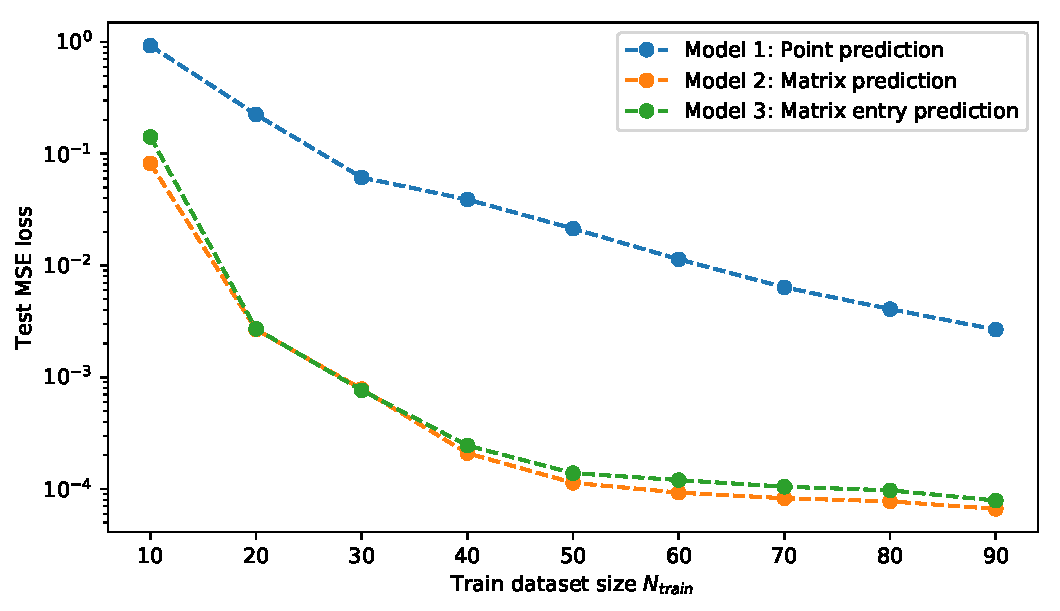
\includegraphics[width=\linewidth]{models}
	\caption{Different model architectures}
	\label{fig:models}
\end{figure}
We can see that while the difference between the behaviours of Model 2 and 3 are quite small, they both perform significantly better than Model 1. This aligns with our expectations, since the latter two models already make use of the knowledge that a rotation can be represented as the multiplication of the point with a matrix that only depends on the rotation angle. Even though both matrix models perform well and almost the same for up to 50 data points, the Model 2 finds a slightly better solution for higher amounts of training data (CHECK IF STILL TRUE FOR 20 RUNS). In order to be able to extract the true effects of the methods we apply, all of the following experiments use one of the well performing models, which we choose to be Model 2. Since it already reaches a Test MSE Loss of almost $10^{-3}$ with 20 training data points and starts to converge only after using more than 6 points, the majority of the following analysis focuses on the interesting region of 10 to 20 as the size of the training dataset. 

\subsection{Penalty method}
\subsubsection{Single minimization problem}
The results of our model trained on solving one minimization problem with 50000 epochs in 2D and a fixed weight $\lambda$ for the detminant physical loss $L_{DET}$ are shown in Figure \ref{fig:pnlty_det}.

\begin{figure}[ht]
	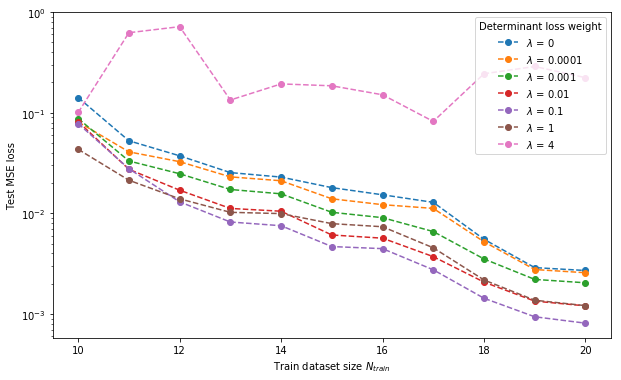
\includegraphics[width=\linewidth]{pnlty_det}
	\caption{Different weights $\lambda$ for $L_{DET}$}
	\label{fig:pnlty_det}
\end{figure}

TODO: Precise characterization once we have 20 runs. (mit werten)\\
The first important result we can conclude from this experiment is the robustness (towards?) the weight of the physical loss, since small weights in a range of at least two orders of magnitude lead to significantly improved results. For smaller values of $\lambda$, the performance converges to the one of $\lambda= 0$, whereas values of $\lambda$ bigger than 1 lead to a heavy focus on satisfying the physical constraint and thus leads to poor results compared to smaller values and $\lambda=0$.

Moreover, we can see that the choice $\lambda = 0.1$ consistently yields to smaller error on the test dataset. It is also important to note that the performance improvement is significant. For example, with only 20 training data points, the physically trained model achieves a Test MSE Loss of xxx, whereas the model trained solely on the train MSE Loss achieves only a value of yyy. \\


Interestingly, utilizing the penalty method leads to higher performance even for larger train datasets. This can be seen in an experiment we did for a wider range of training dataset sizes in Figure APPENDIX FIGURE.\\
We observe similar qualitative behaviour when applying the method for the 3D-rotation, as displayed in Figure APPENDIX FIGURE.\\

\clearpage

